%% chapter 4 Species-level traits - responses to land use and climate-change sensititivy

\section*{Keywords}

\section*{Abstract}

\section{Introduction}

%% Figure 1 = framework

\begin{figure}[h!]
\centering
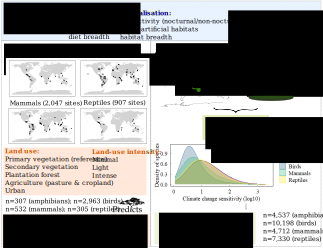
\includegraphics[scale=0.55]{figures/Chapter4/Figure1}
\caption[Framework of the study]{\textbf{Framework of the study.} \textbf{(a)} I collected ecological trait data and geographical range areas across terrestrial vertebrates (termed `ecological characteristics'). I then used two independent approaches to assess the influence of these characteristics on species responses to land-use and on species climate-change  sensitivity. \textbf{(b)} To assess the influence of traits on responses to land use and land-use intensity in each vertebrate class, I combined the ecological characteristics with the PREDICTS database. \textbf{(c)} To estimate species sensitivity to climate change, I used the CENFA framework \citep{Rinnan2019}, which relies on the combination of species’ distributions with climatic variables to estimate sensitivity from properties of the species’ climatic niche space. I then built class-specific models to assess whether the ecological characteristics were associated with  species sensitivity to climate change.}
\label{chap4_fig1}
\end{figure}

\clearpage

\section{Methods}

%% Figure 2 = assessing effects 
\begin{figure}[h!]
\centering
\includegraphics[scale=1.7]{figures/Chapter4/Figure2}
\caption[]{}
\label{chap4_fig2}
\end{figure}


\section{Results}

\section{Discussion}
